La interpretación astrofísica de los grafos Mapper se plantea como una lectura de regiones candidatas, no como una clasificación definitiva de exoplanetas. En este reporte, una región se considera astrofísicamente interesante si combina tres condiciones: coherencia física u orbital, baja dependencia de imputación y baja concentración observacional. Por el contrario, una región debe interpretarse con cautela si depende de variables altamente imputadas, si está dominada por un método de descubrimiento o si su estructura solo aparece bajo una elección específica del lente.

Esta distinción es central porque Mapper puede producir grafos visualmente ricos sin que todas sus regiones tengan el mismo nivel de evidencia científica. Un nodo grande, una rama o un ciclo no equivalen automáticamente a una población planetaria real. La interpretación depende de qué variables sostienen esa región, qué tan observados o imputados son sus valores, y si la composición del nodo está asociada con el proceso de descubrimiento.

Las estructuras con interpretación física más directa aparecen en los grafos \texttt{phys\_min\_pca2\_cubes10\_overlap0p35}, \texttt{phys\_density\_pca2\_cubes10\_overlap0p35} y en algunas regiones de los espacios conjuntos. Estos grafos organizan planetas mediante radio, masa y, en algunos casos, densidad. Por ello, permiten inspeccionar regiones compatibles con diferencias de escala planetaria: planetas pequeños, sub-Neptunos, Neptunos o sub-jovianos y gigantes. Sin embargo, estas etiquetas deben entenderse como apoyos interpretativos. Un nodo dominado por una clase de radio no equivale a una clase planetaria definitiva; indica una región local con coherencia física bajo las variables usadas.

Las tablas de interpretación nodal utilizan etiquetas como \texttt{rocky\_size}, \texttt{sub\_neptune\_size}, \texttt{neptune\_or\_sub\_jovian\_size} y \texttt{jovian\_size}. Estas etiquetas permiten identificar nodos dominados por clases de radio y ayudan a leer gradientes físicos dentro del grafo. En particular, los espacios físicos y conjuntos sugieren regiones diferenciadas entre planetas de tamaño pequeño o intermedio y planetas gigantes. Esta separación no debe interpretarse como una frontera rígida; Mapper sugiere una organización gradual, donde pueden existir transiciones entre poblaciones.

\begin{figure}[H]
\centering
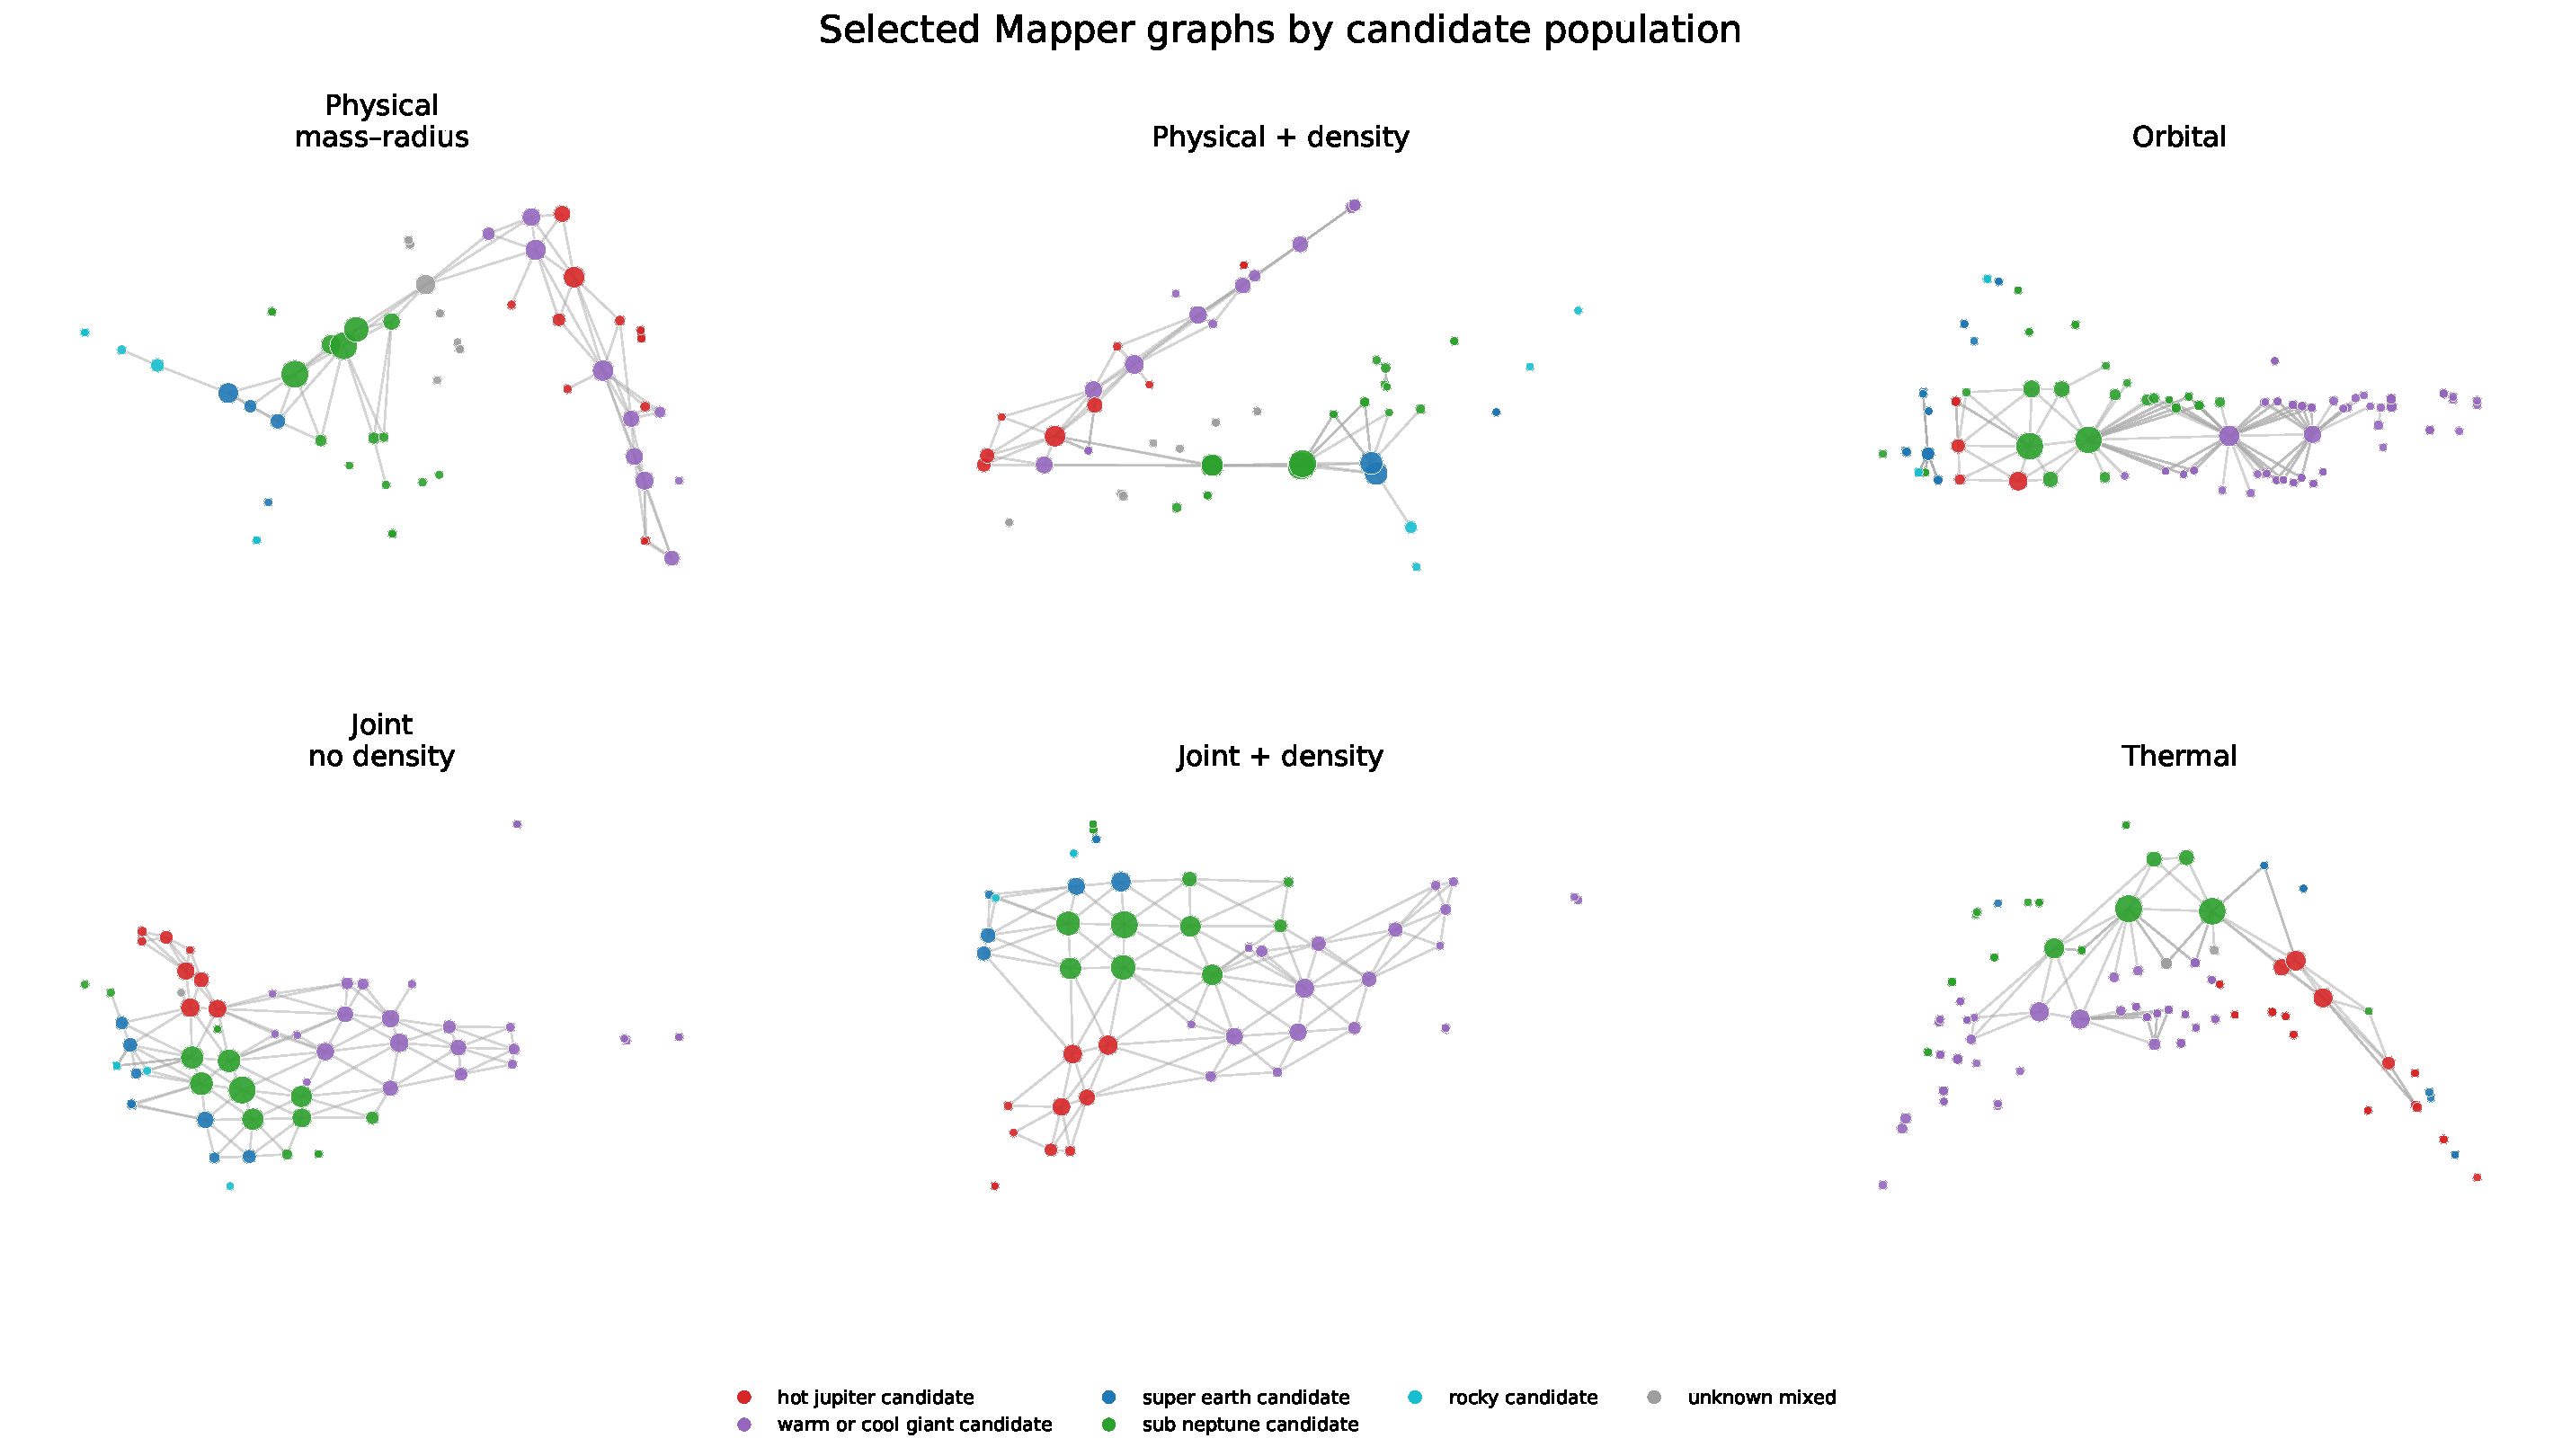
\includegraphics[width=0.92\linewidth]{figures/astro_main_graphs_by_candidate_population.pdf}
\caption{Grafos principales coloreados por población física heurística. La visualización permite evaluar si las regiones de Mapper están dominadas por poblaciones candidatas o si la señal física aparece mezclada dentro de los grafos. La presencia de grandes regiones dominadas por una misma etiqueta debe interpretarse como coherencia heurística local, no como una clase planetaria definitiva.}
\label{fig:main_graphs_by_population}
\end{figure}

\begin{figure}[H]
\centering
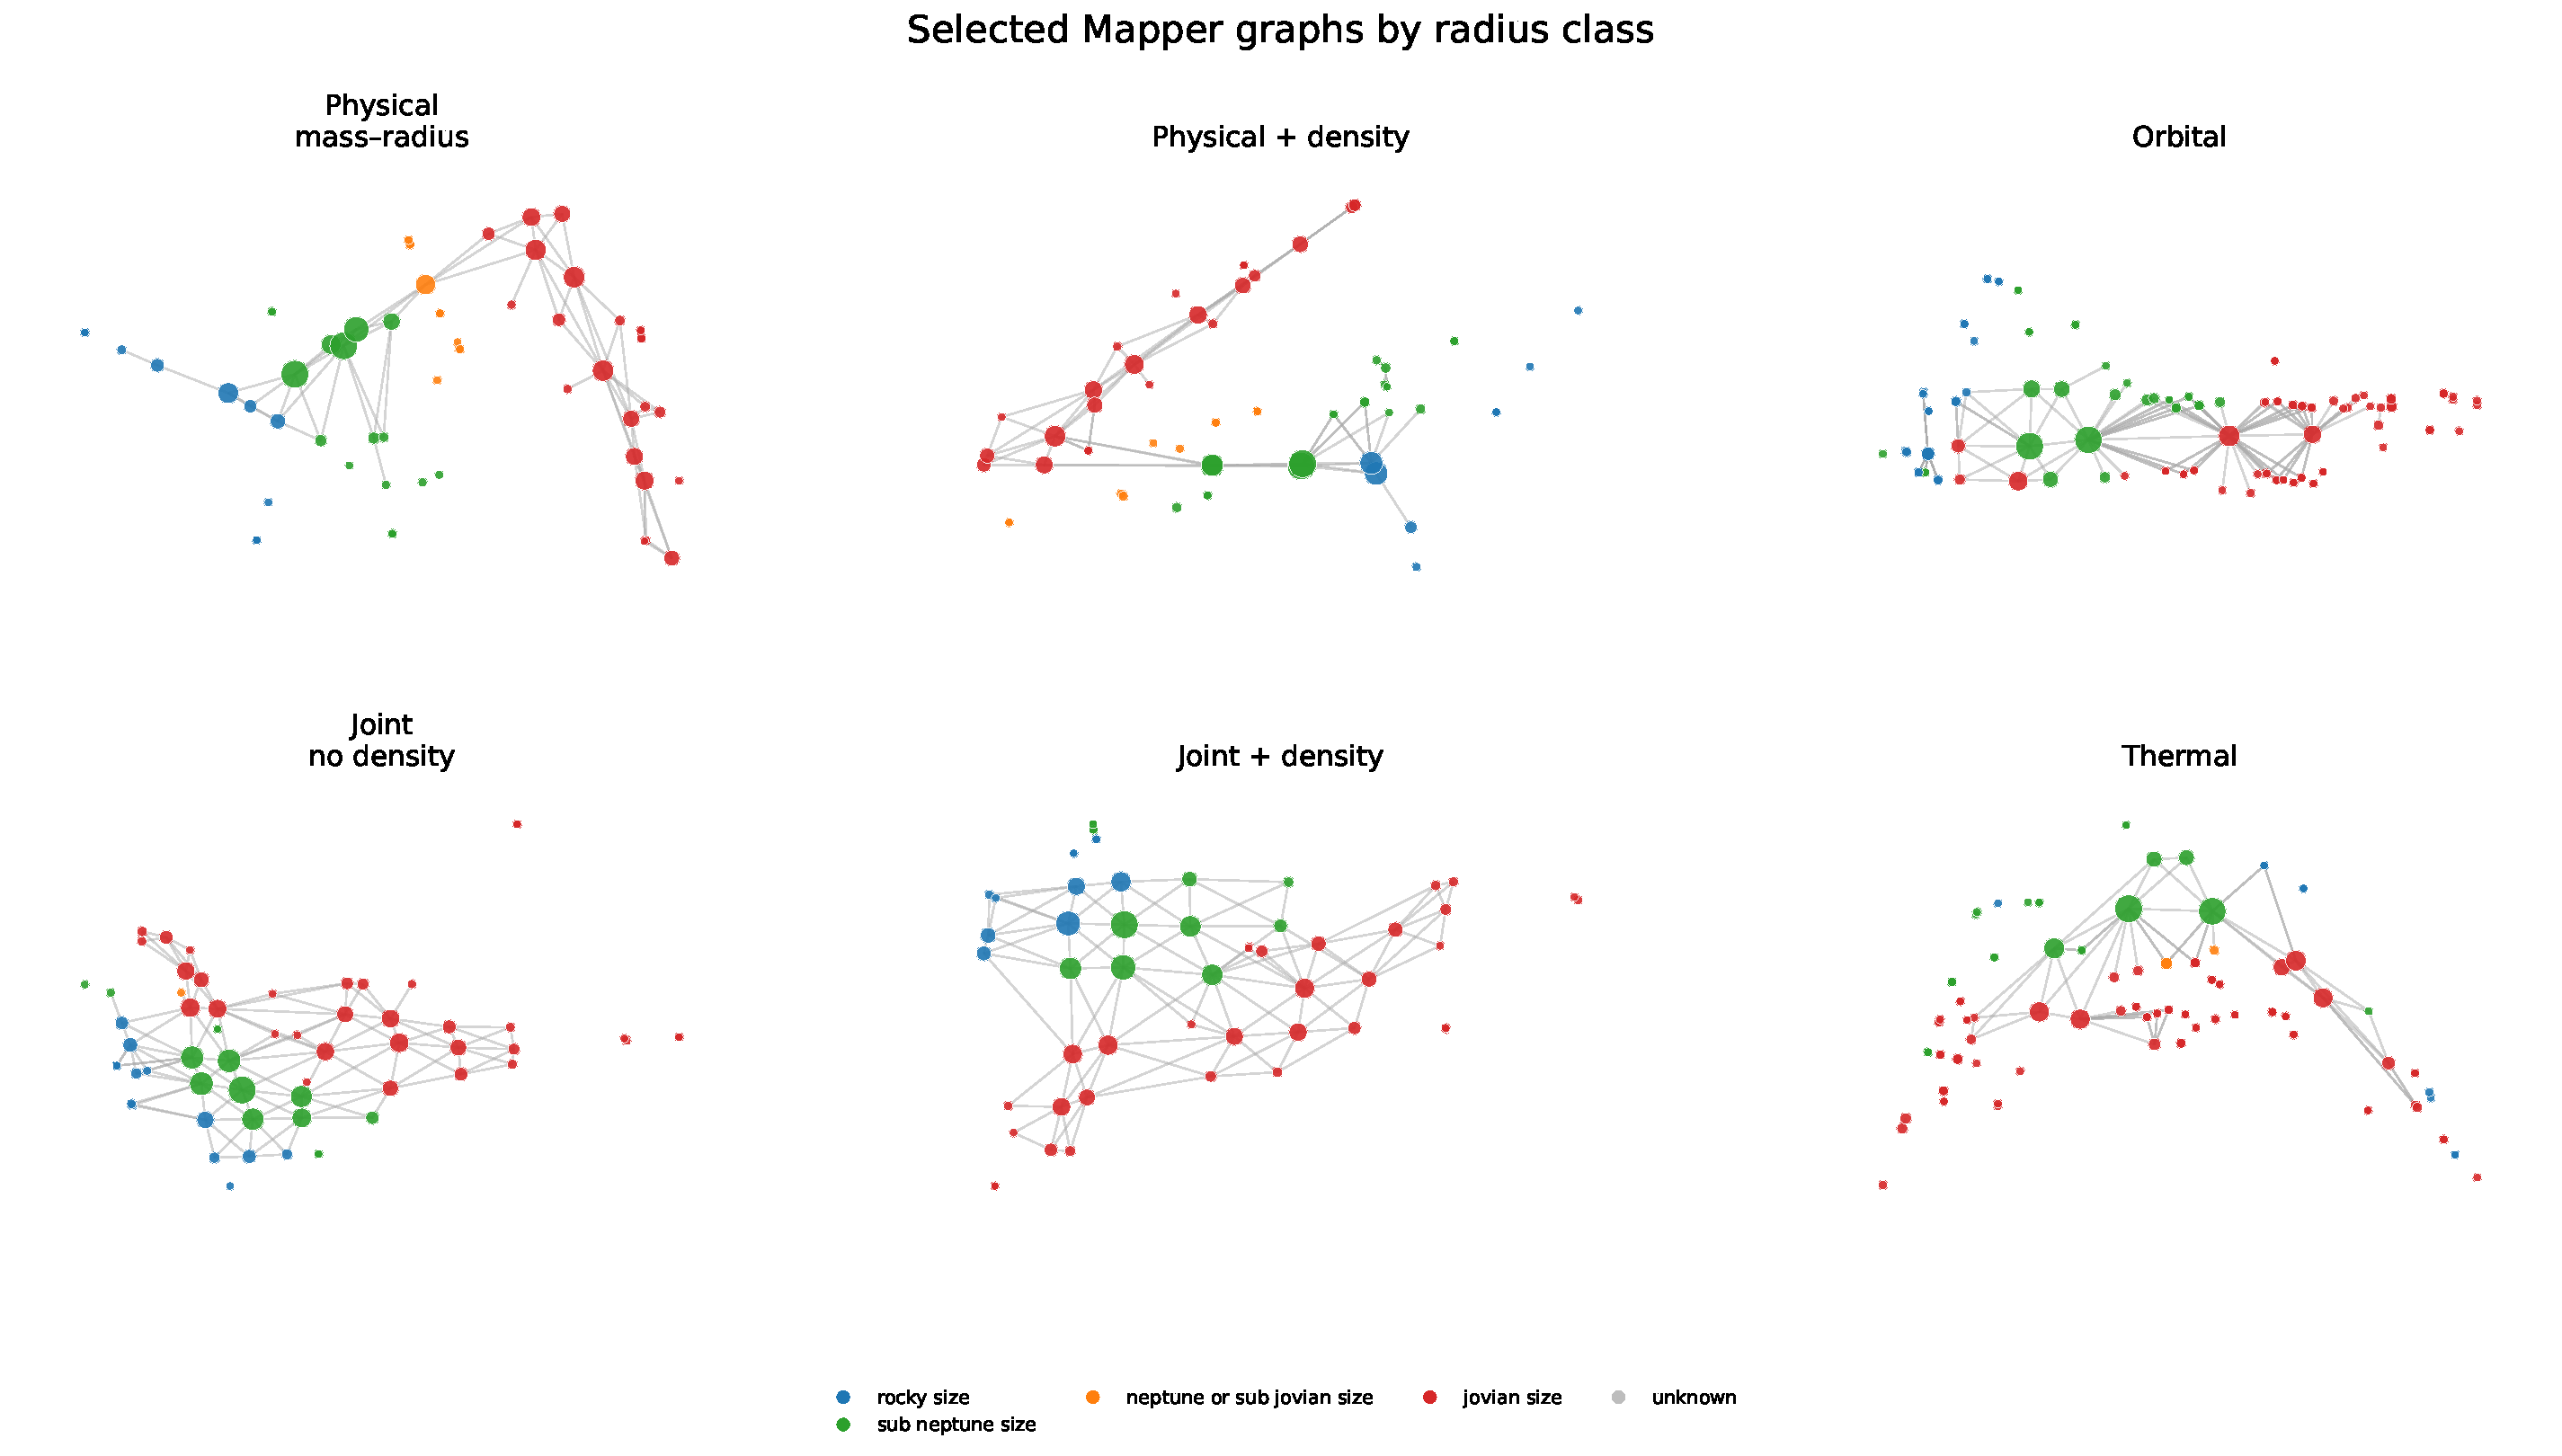
\includegraphics[width=0.92\linewidth]{figures/astro_main_graphs_by_radius_class.pdf}
\caption{Grafos principales coloreados por clase de radio dominante. Esta version separa visualmente regiones \texttt{rocky\_size}, \texttt{sub\_neptune\_size}, \texttt{neptune\_or\_sub\_jovian\_size} y \texttt{jovian\_size}, lo que permite revisar si la estructura local coincide con gradientes de tamano planetario.}
\label{fig:astro_main_graphs_by_radius_class}
\end{figure}

La Figura~\ref{fig:main_graphs_by_population} muestra que las etiquetas heurísticas pueden ayudar a ubicar regiones físicamente plausibles, pero también evidencia una limitación importante: en varios grafos la señal visual aparece concentrada en regiones grandes y no necesariamente separada en múltiples poblaciones limpias. Esto refuerza la idea de que la interpretación debe hacerse por región y no solo por inspección global del grafo. Una población heurística dominante puede indicar coherencia física local, pero todavía debe cruzarse con imputación y sesgo observacional.

Además de las clases por radio, los nodos físicos resumen valores medios y medianos de \texttt{pl\_rade}, \texttt{pl\_bmasse} y \texttt{pl\_dens}. Esto permite leer gradientes de tamaño, masa y densidad entre regiones del grafo. La densidad, sin embargo, requiere una interpretación particular. Aunque \texttt{pl\_dens} es físicamente útil para distinguir planetas compactos de planetas de baja densidad, muchos de sus valores fueron derivados a partir de masa y radio. Por ello, cuando se usa junto con \texttt{pl\_rade} y \texttt{pl\_bmasse}, no debe tratarse como evidencia completamente independiente.

\begin{figure}[H]
\centering
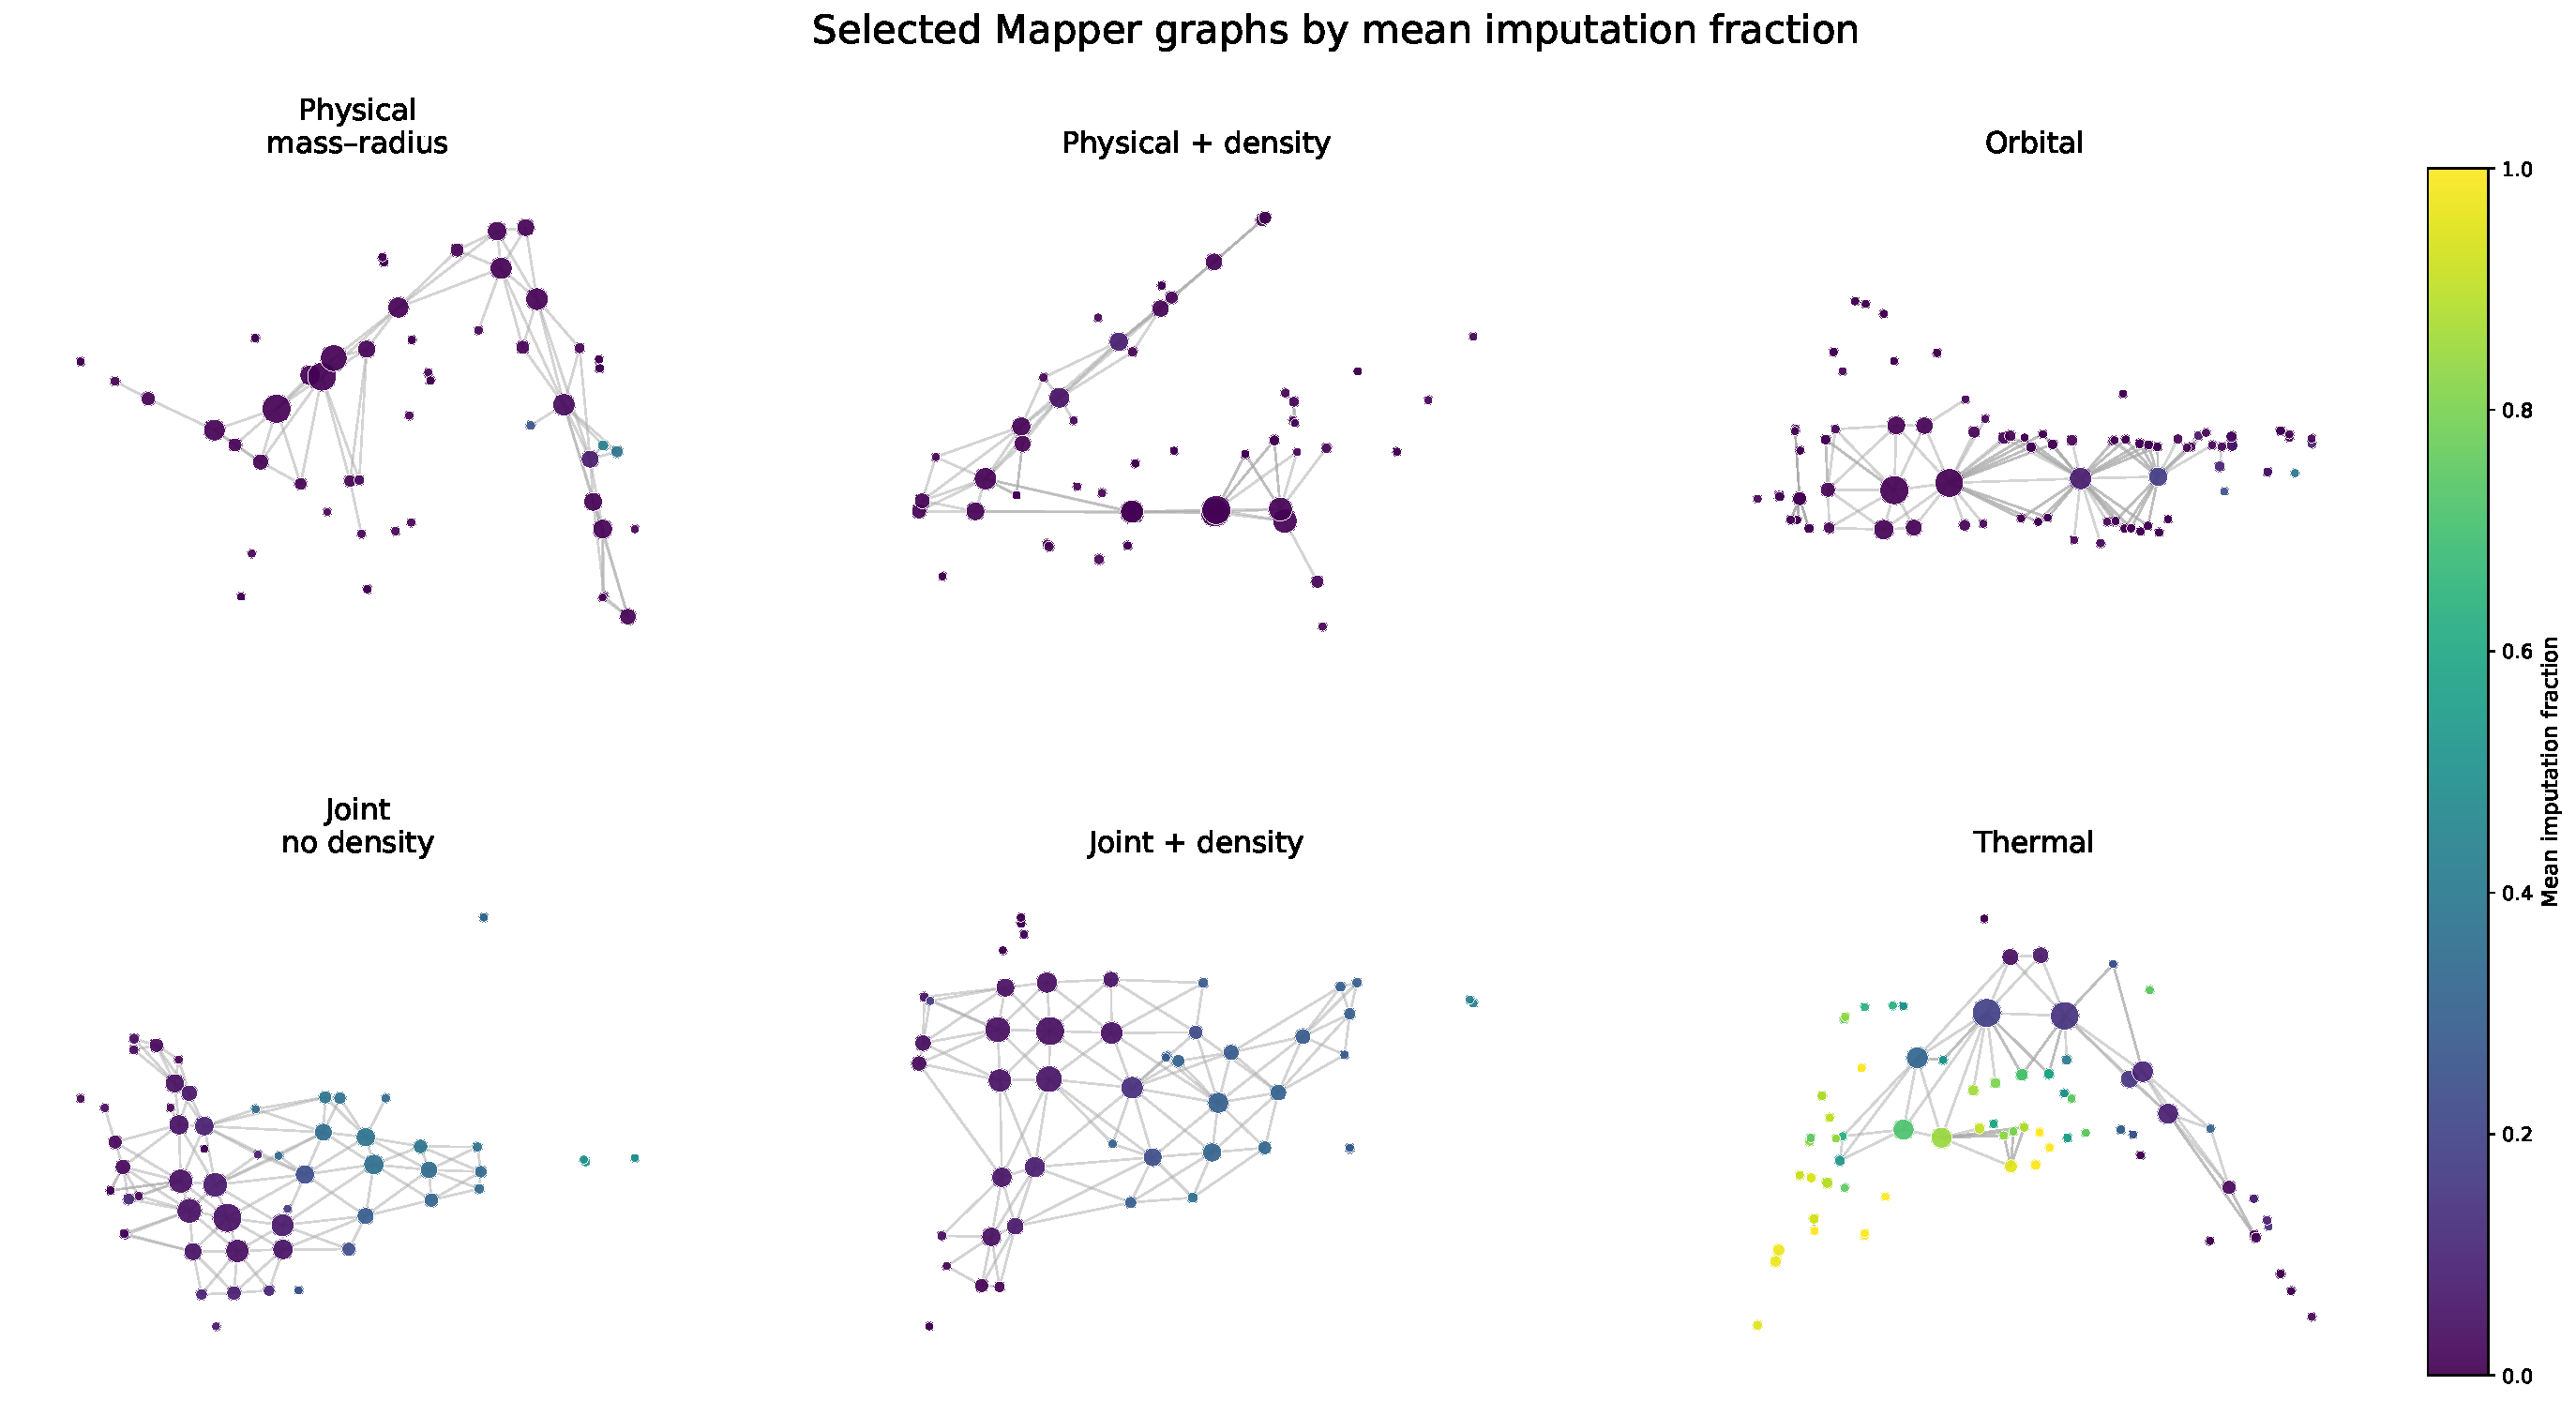
\includegraphics[width=0.92\linewidth]{figures/astro_main_graphs_by_imputation_fraction.pdf}
\caption{Grafos principales coloreados por fracción de imputación o trazabilidad de origen de datos. Esta visualización permite distinguir regiones sostenidas principalmente por datos observados de regiones con mayor dependencia de valores imputados o derivados. En particular, ayuda a interpretar con cautela los espacios que incorporan variables térmicas o densidad derivada.}
\label{fig:main_graphs_by_imputation}
\end{figure}

La Figura~\ref{fig:main_graphs_by_imputation} muestra por qué la interpretación astrofísica no puede separarse de la trazabilidad de datos. Una región puede parecer estructurada, pero si su color indica alta imputación o alta proporción de valores derivados, la evidencia que sostiene esa región es más débil. Esta observación es especialmente relevante para el espacio térmico y para los grafos que incorporan \texttt{pl\_dens}. En esos casos, la estructura observada puede ser útil como señal exploratoria, pero no debe elevarse directamente a conclusión física fuerte.

Los resultados medidos sugieren que la densidad actúa más como una variable de regularización que como una fuente nueva de ramificación topológica. Al comparar el espacio físico mínimo con el espacio físico con densidad, \(\beta_1\) baja de 54 en \texttt{phys\_min} a 52 en \texttt{phys\_density}. De manera similar, en el espacio conjunto \(\beta_1\) baja de 81 en \texttt{joint\_no\_density} a 77 en \texttt{joint}. Esta disminución indica que agregar \texttt{pl\_dens} compacta u ordena parte del espacio, en lugar de crear más ciclos o ramas. Por esta razón, los grafos con densidad se leen como controles metodológicos y no como evidencia independiente de una estructura física adicional.

La estructura orbital es el resultado más importante del análisis. El grafo \texttt{orbital\_pca2\_cubes10\_overlap0p35} tiene 124 nodos, 196 aristas, \(\beta_1=96\) e imputación media nodal de 0.011. Esta combinación lo vuelve el candidato más fuerte para inspección científica: muestra una topología rica y, al mismo tiempo, depende poco de valores imputados. Como este grafo usa \texttt{pl\_orbper} y \texttt{pl\_orbsmax}, su estructura es compatible con una organización del catálogo según escala orbital, es decir, por periodo y distancia media a la estrella.

Dentro de la lectura orbital, las etiquetas como \texttt{short\_period}, \texttt{intermediate\_period} y \texttt{long\_period} permiten distinguir regiones asociadas con distintos regímenes orbitales. Las regiones de periodo corto son físicamente interpretables porque corresponden a planetas cercanos a su estrella, pero también deben leerse con cuidado: los métodos de tránsito tienden a detectar con mayor facilidad planetas de periodos cortos. Por eso, una región dominada por planetas de periodo corto puede reflejar tanto una propiedad orbital real como un sesgo de observación.

También aparecen regiones compatibles con órbitas más amplias, incluyendo etiquetas como \texttt{long\_period} o poblaciones candidatas como \texttt{long\_period\_giant\_candidate}. Estas regiones son científicamente interesantes porque pueden señalar arquitecturas orbitales distintas, pero su composición también puede estar asociada con métodos específicos de detección, como imagen directa, microlente o velocidad radial. En consecuencia, la interpretación orbital debe mantenerse como una lectura mixta: el grafo muestra estructura, pero esa estructura puede combinar arquitectura orbital y selección observacional.

El espacio térmico presenta un caso distinto. El grafo \texttt{thermal\_pca2\_cubes10\_overlap0p35} tiene \(\beta_1=67\), lo que indica una estructura no trivial. Sin embargo, su imputación media nodal es 0.588 y la fracción de nodos con alta imputación es 0.719. Esto debilita significativamente su interpretación física. El espacio térmico puede sugerir gradientes energéticos relacionados con \texttt{pl\_insol} y \texttt{pl\_eqt}, pero no debe usarse como evidencia física fuerte sin una auditoría adicional de imputación. En este reporte, el grafo térmico funciona principalmente como caso de cautela metodológica: una estructura puede ser visualmente rica y, aun así, estar sostenida por datos completados estadísticamente.

Los espacios conjuntos permiten observar cómo se combinan propiedades físicas, orbitales y térmicas. En particular, \texttt{joint\_no\_density\_pca2\_cubes10\_overlap0p35} combina radio, masa, periodo, semieje mayor, insolación y temperatura de equilibrio. Este grafo tiene \(\beta_1=81\) e imputación media de 0.176. La complejidad del espacio conjunto sugiere que algunas regiones pueden alinear propiedades físicas y orbitales, pero la presencia de variables térmicas aumenta el riesgo por imputación. Por tanto, estas regiones se leen como candidatas mixtas: pueden ser astrofísicamente interesantes, pero requieren más cautela que el grafo orbital.

La síntesis final de regiones refuerza esta lectura cautelosa. La evidencia astrofísica más útil aparece cuando una región combina baja imputación, coherencia física u orbital y baja concentración observacional. Bajo estos criterios, los resultados finales identifican 10 nodos etiquetados como \texttt{physical}. Esto indica que existen regiones con evidencia relativamente limpia de interpretación física, pero son pocas en comparación con el total de regiones estructuradas. En contraste, muchas regiones quedan clasificadas como \texttt{mixed}: 240 nodos y 36 componentes. Esto significa que presentan algún patrón físico u orbital, pero también una señal observacional relevante.

Este resultado es importante porque cambia la lectura del proyecto. Si se observara únicamente la complejidad de los grafos, podría parecer tentador hablar de familias planetarias o de clases emergentes. Sin embargo, el predominio de regiones \texttt{mixed} muestra que la estructura observada no es puramente astrofísica ni puramente observacional. En muchos casos, Mapper detecta regiones donde la señal física u orbital está mezclada con método de descubrimiento, imputación, derivaciones físicas o sensibilidad metodológica.

Por esta razón, las regiones físicamente interpretables deben leerse como candidatas para inspección posterior. Una región con alta pureza de clase física, baja imputación y baja concentración por \texttt{discoverymethod} puede considerarse una candidata fuerte. En cambio, una región con coherencia física pero alta asociación con método de descubrimiento debe clasificarse como mixta. Esta clasificación no debilita el proyecto; al contrario, muestra por qué la auditoría era necesaria. Sin ella, una región estructurada podría haberse interpretado erróneamente como una familia física pura.

Una pregunta central de esta sección es si las regiones observadas pueden interpretarse como clases planetarias reales. La respuesta metodológica es no. Las regiones Mapper deben leerse como candidatos interpretativos, no como clases definitivas. Un nodo puede estar dominado por planetas pequeños, por gigantes o por un régimen orbital particular, pero su significado depende de la imputación, de la composición observacional y de la sensibilidad del lente. Esta cautela es especialmente importante porque la auditoría de sesgo observacional mostró asociación con \texttt{discoverymethod}. En el grafo orbital, por ejemplo, la pureza ponderada observada por método fue 0.842, el NMI observado fue 0.254 y el valor empírico de la prueba por permutación fue \(p=0.001\). Por ello, no se puede descartar que parte de la estructura orbital refleje sesgo de descubrimiento.

La dependencia de imputación también varía fuertemente entre espacios. El patrón orbital es menos dependiente de imputación que el térmico: la imputación media nodal del grafo orbital es 0.011, mientras que la del grafo térmico es 0.588. El espacio físico mínimo también tiene baja imputación, con 0.017, mientras que el espacio conjunto sin densidad tiene una imputación moderada de 0.176. Estas diferencias justifican que el grafo orbital y el físico mínimo se consideren más confiables que el térmico para interpretación inicial.

Finalmente, existen artefactos para tres lentes: \texttt{pca2}, \texttt{domain} y \texttt{density}. Sin embargo, la interpretación activa del reporte se basa en \texttt{pca2}. Las otras lentes funcionan como sensibilidad metodológica, no como confirmación definitiva. Además, como los artefactos reconciliados no constituyen una grilla completa de \texttt{n\_cubes} y \texttt{overlap}, la persistencia de patrones entre lentes debe leerse con cuidado. Hay evidencia para comparar lentes bajo una cubierta fija, pero no suficiente para afirmar robustez completa frente a todos los hiperparámetros de Mapper.

\subsection*{Visualizaciones astrofisicas complementarias}

Las siguientes figuras usan el mismo estilo de renderizado limpio que la sintesis final, pero colorean los grafos por etiquetas interpretativas astrofisicas. Estas visualizaciones no definen clases finales; sirven para ubicar regiones candidatas y compararlas con la auditoria de imputacion y sesgo observacional.

\begin{figure}[H]
\centering
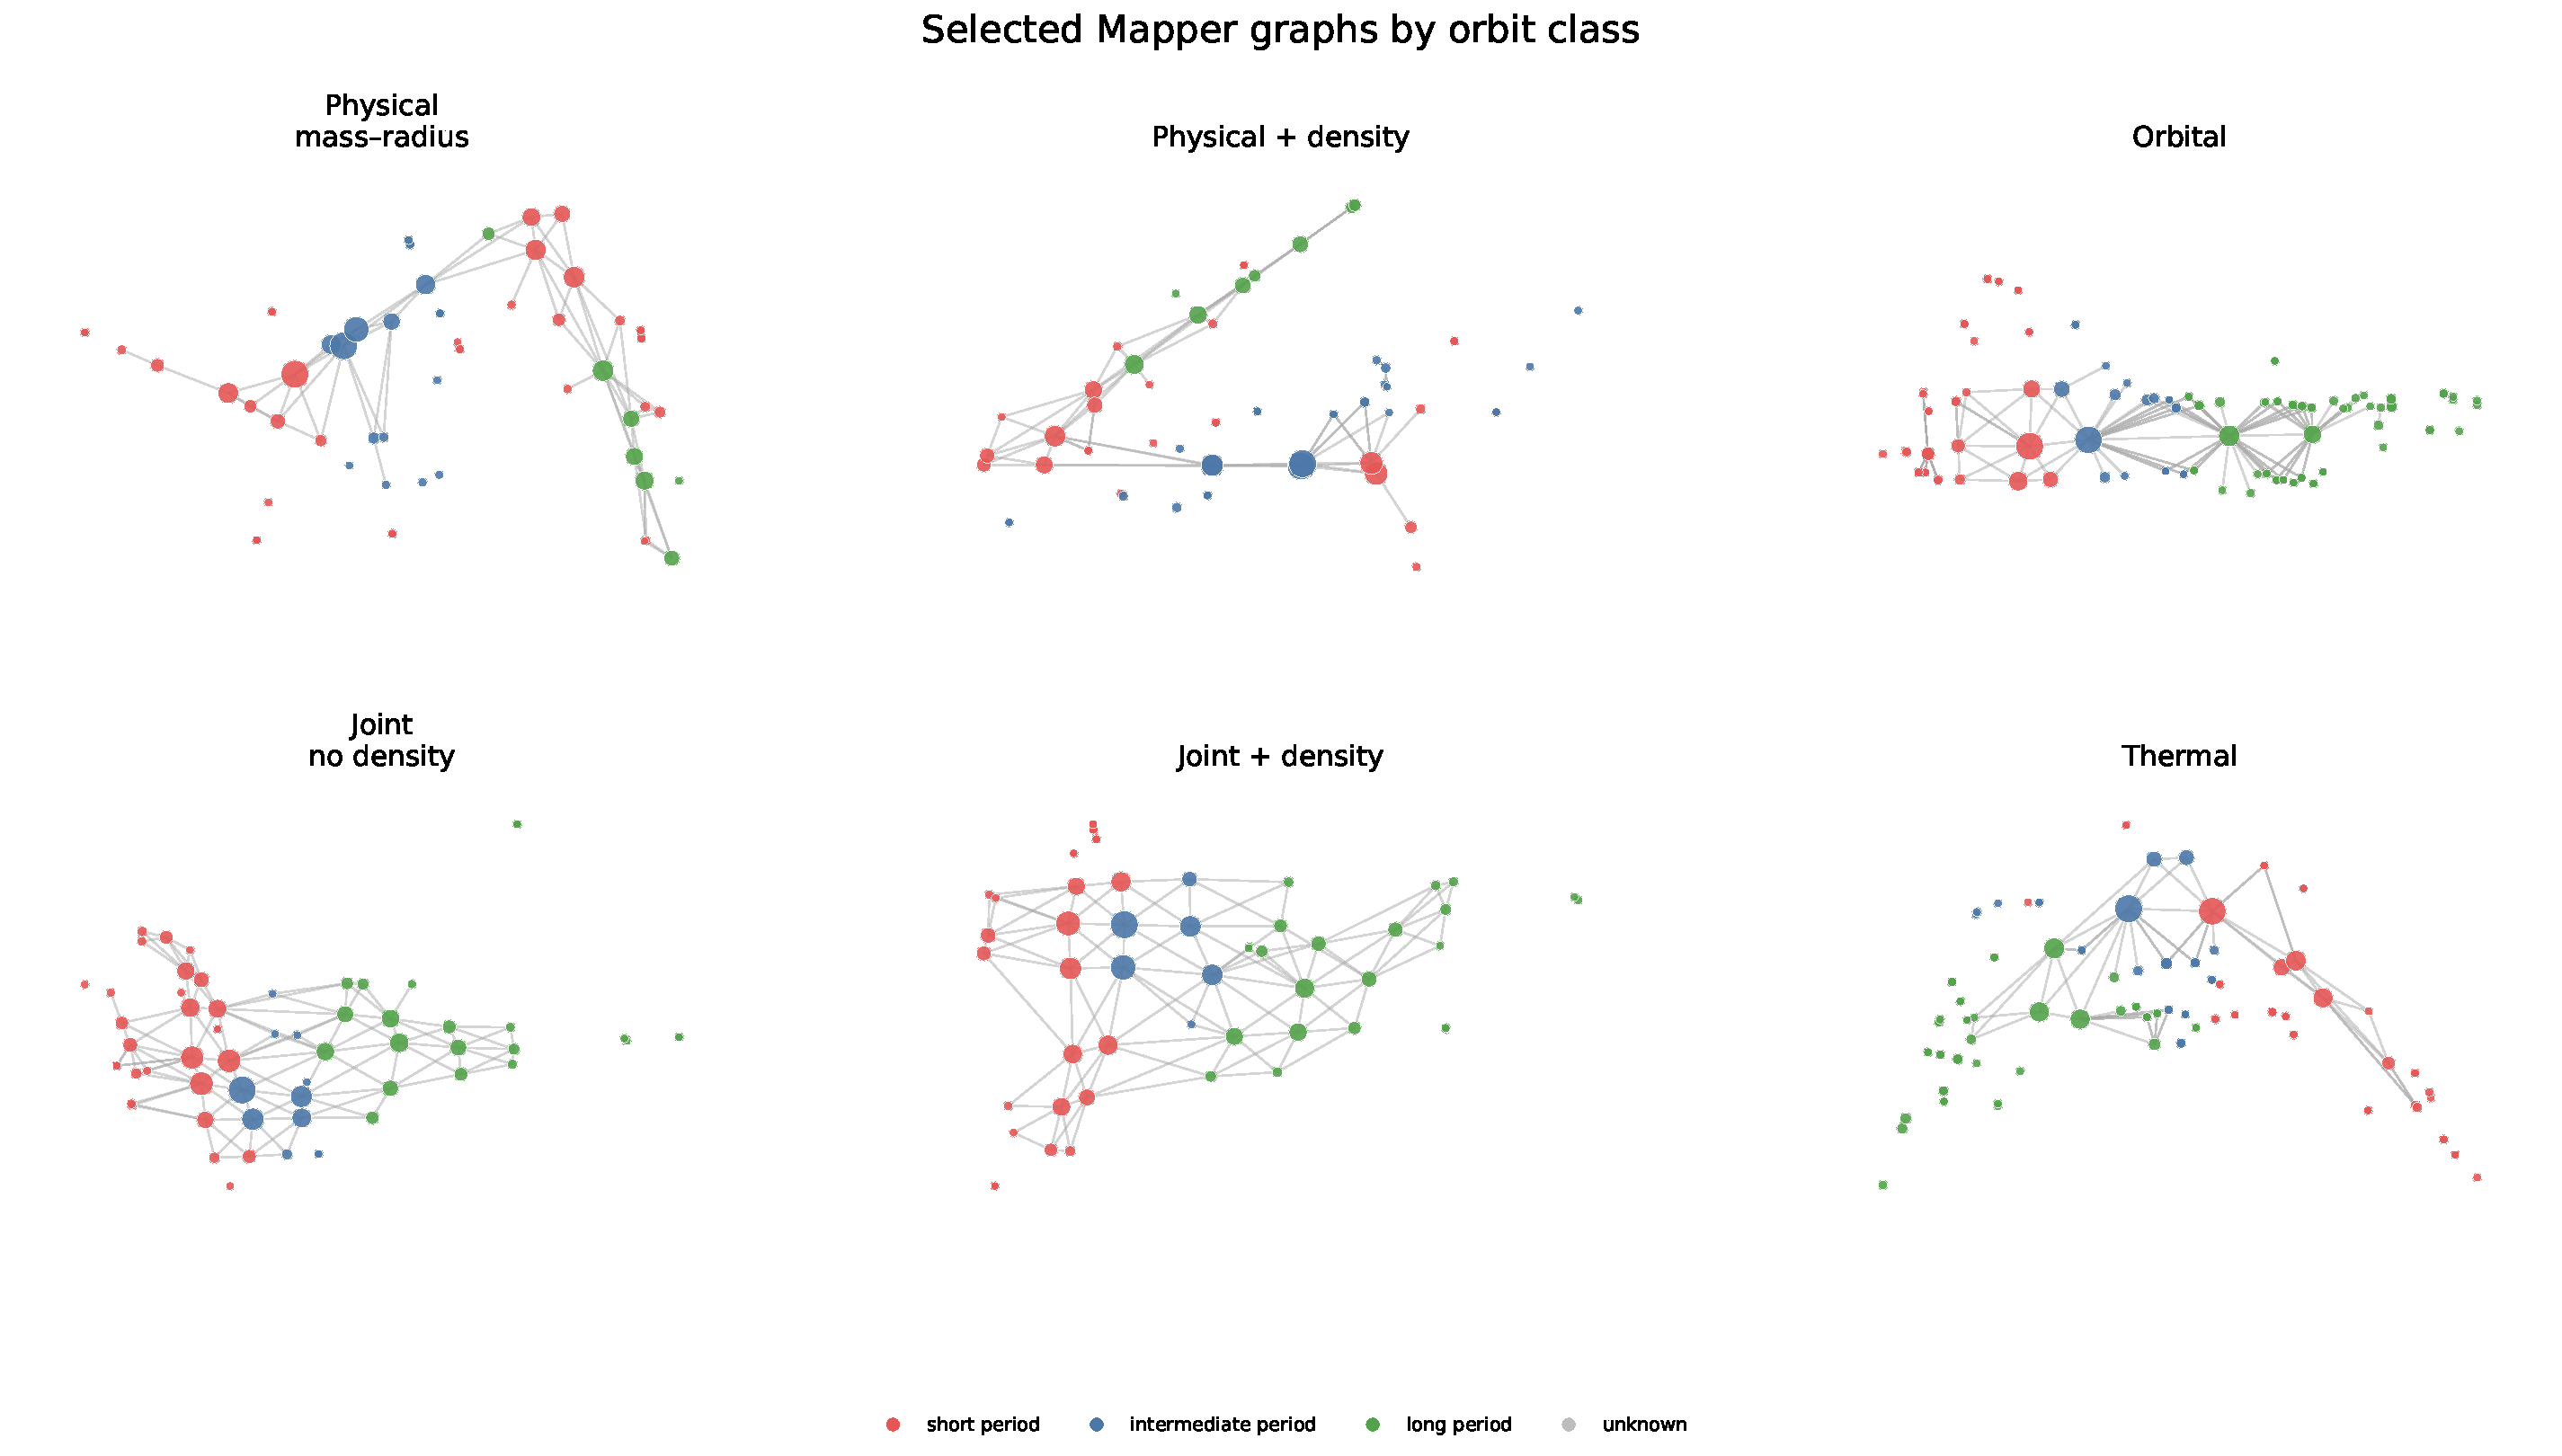
\includegraphics[width=0.92\linewidth]{figures/astro_main_graphs_by_orbit_class.pdf}
\caption{Grafos principales coloreados por clase orbital dominante. La figura permite comparar regiones de periodo corto, intermedio y largo en los espacios seleccionados.}
\label{fig:astro_main_graphs_by_orbit_class}
\end{figure}

\begin{figure}[H]
\centering
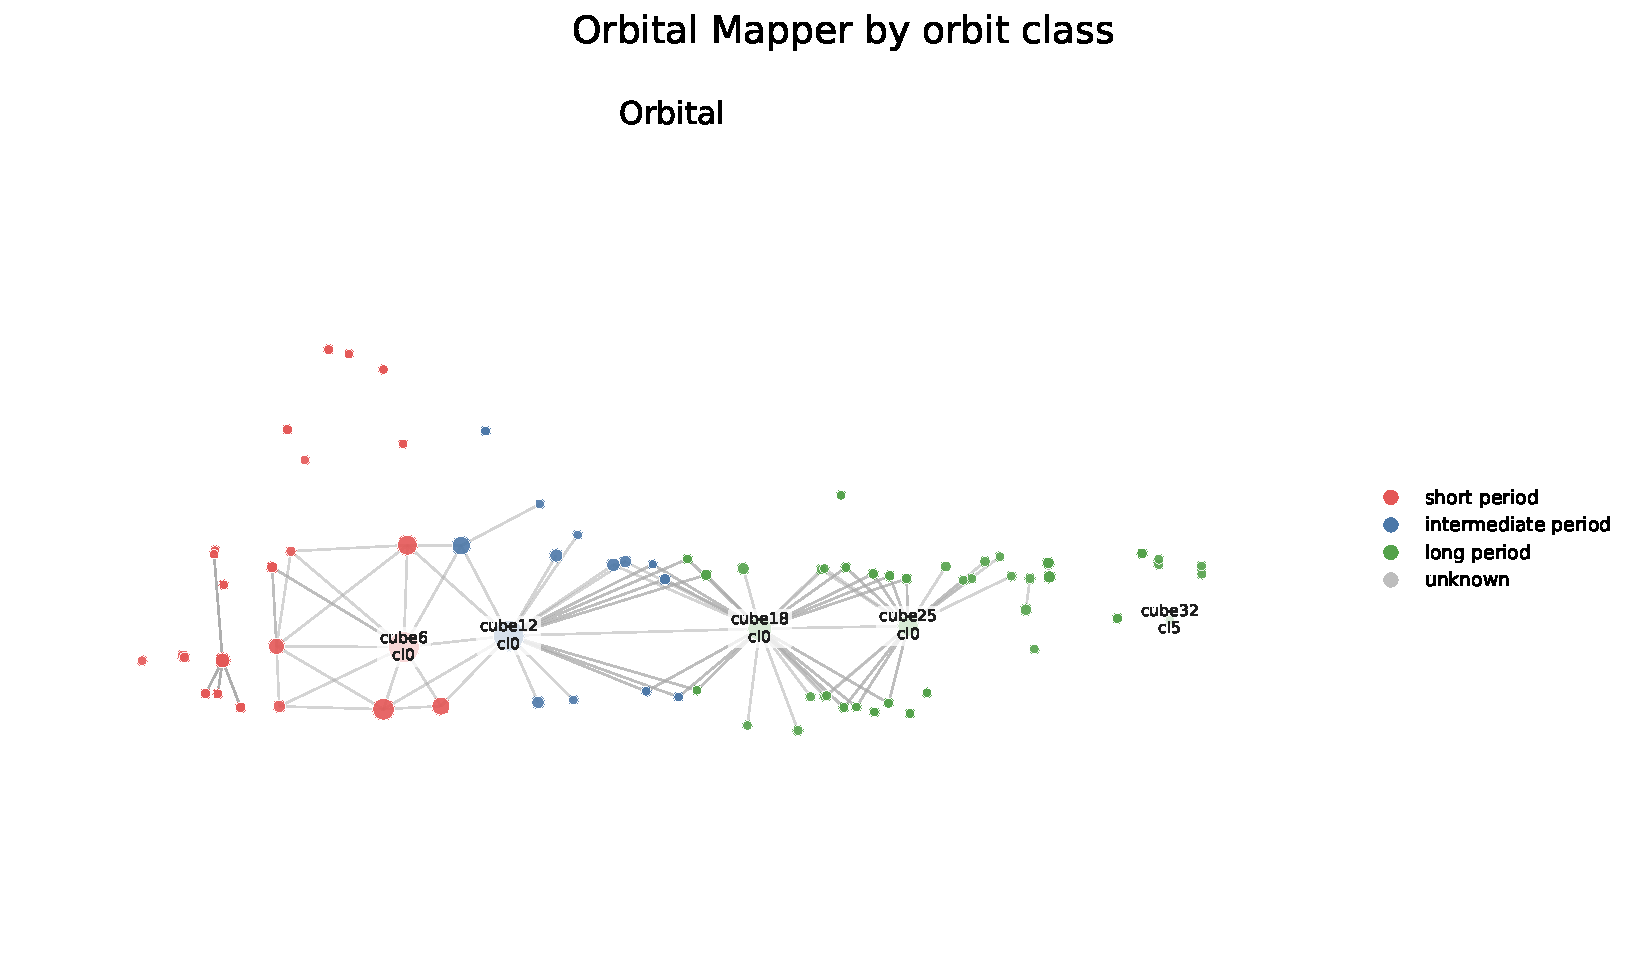
\includegraphics[width=0.78\linewidth]{figures/astro_orbital_graph_by_orbit_class.pdf}
\caption{Grafo orbital coloreado por clase orbital dominante. La figura muestra la transicion visual entre regiones de periodo corto, intermedio y largo.}
\label{fig:astro_orbital_graph_by_orbit_class}
\end{figure}

\begin{figure}[H]
\centering
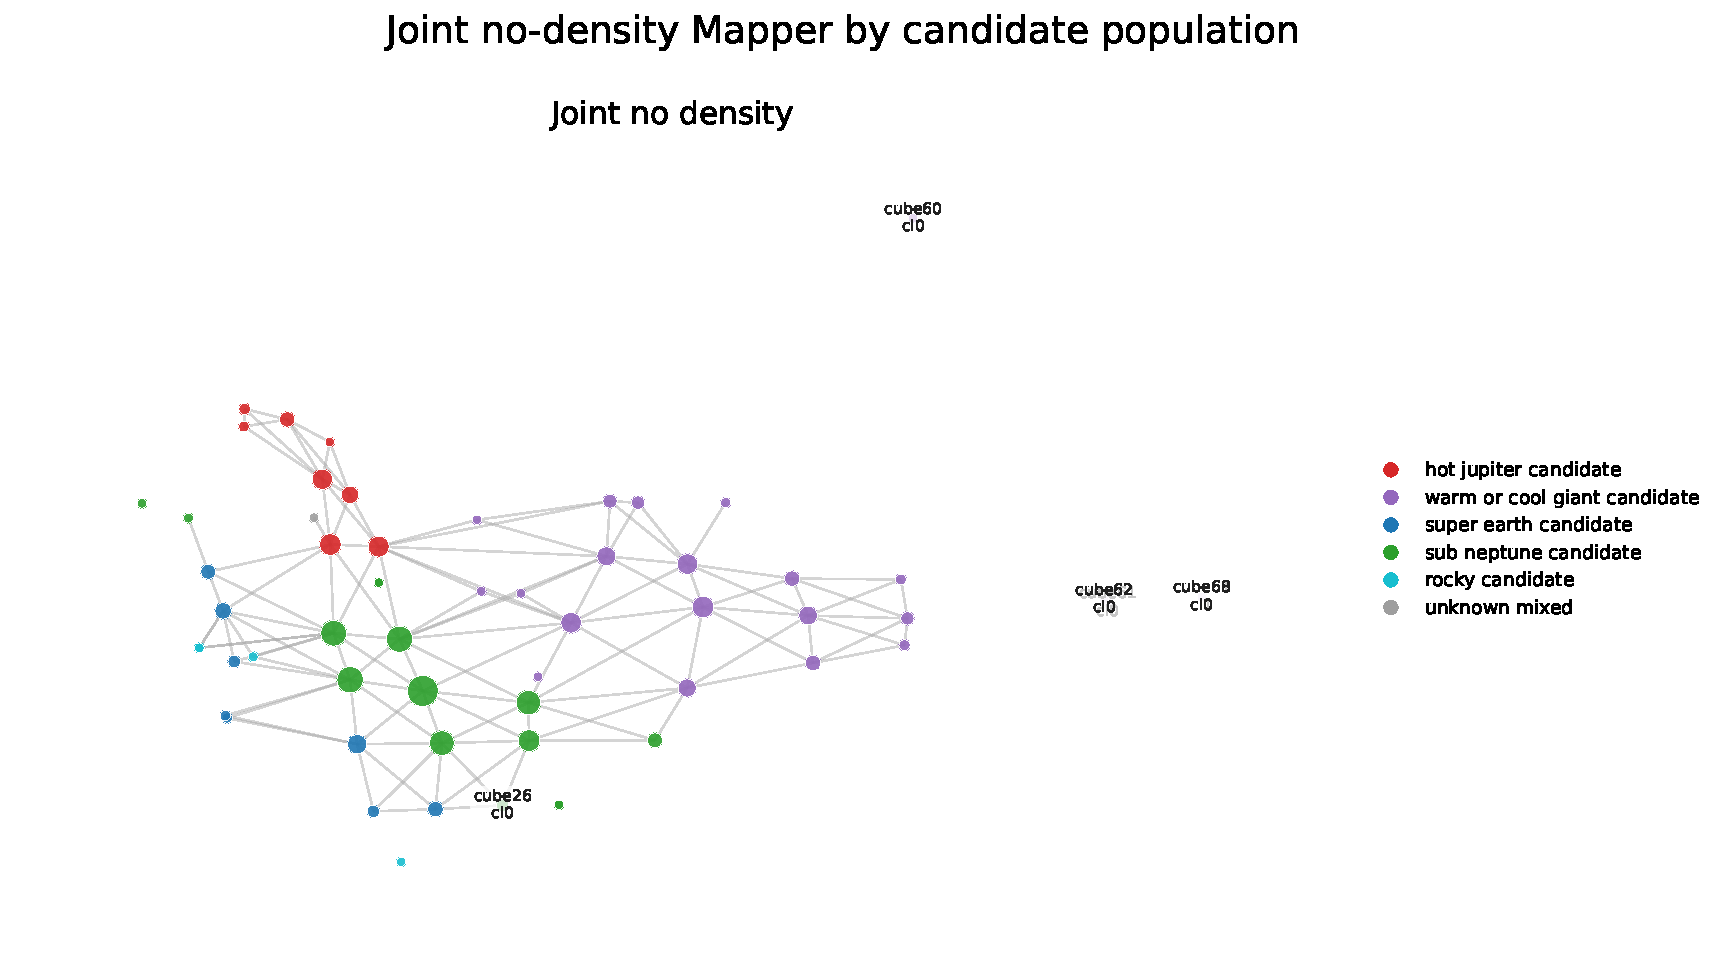
\includegraphics[width=0.78\linewidth]{figures/astro_joint_no_density_graph_by_candidate_population.pdf}
\caption{Grafo conjunto sin densidad coloreado por poblacion candidata. Esta vista ayuda a revisar donde se alinean radio, masa, orbita y variables termicas sin introducir la densidad derivada como coordenada adicional.}
\label{fig:astro_joint_no_density_graph_by_candidate_population}
\end{figure}

\begin{figure}[H]
\centering
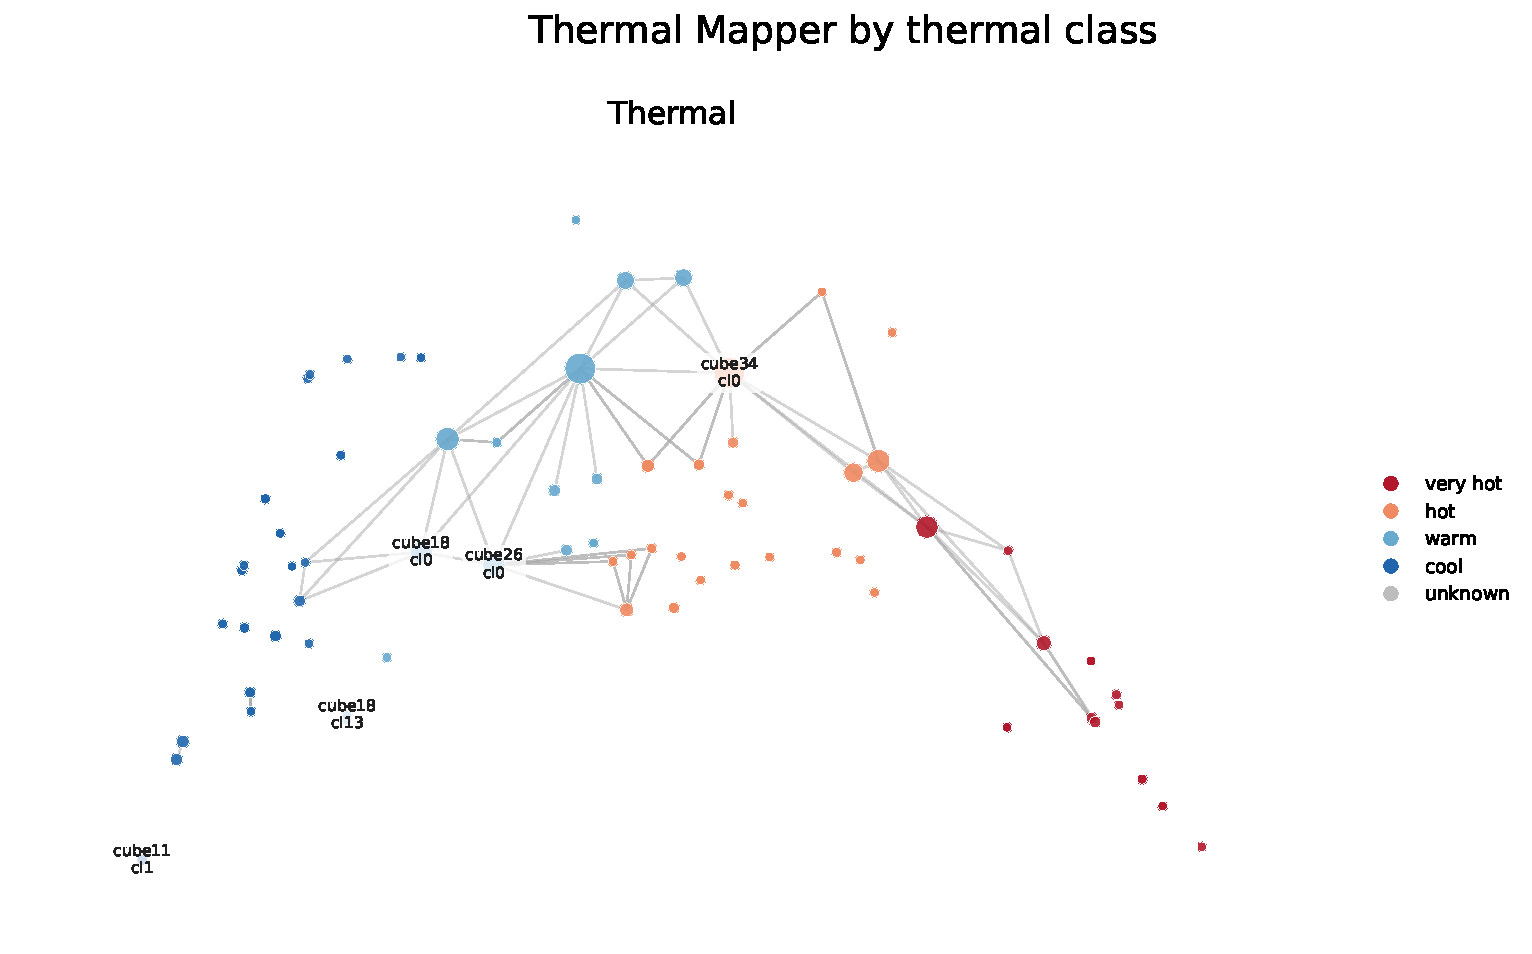
\includegraphics[width=0.78\linewidth]{figures/astro_thermal_graph_by_thermal_class.pdf}
\caption{Grafo termico coloreado por clase termica dominante. Aunque aparecen gradientes de temperatura, la alta imputacion del espacio termico obliga a leer esta estructura como evidencia cautelosa.}
\label{fig:astro_thermal_graph_by_thermal_class}
\end{figure}

\begin{table}[H]
\centering
\scriptsize
\caption{Comparacion de espacios de variables para los artefactos existentes.}
\label{tab:space_comparison}
\begin{adjustbox}{max width=\linewidth}
\begin{tabular}{llrrrr}
\toprule
feature\_space & lens & beta\_1 & n\_nodes & n\_edges & mean\_node\_imputation \\
\midrule
joint & density & 153 & 117 & 260 & 0.106 \\
joint\_no\_density & density & 134 & 109 & 233 & 0.142 \\
orb\_thermal & density & 138 & 121 & 246 & 0.255 \\
orbital & density & 144 & 178 & 297 & 0.030 \\
phys\_density & density & 52 & 78 & 109 & 0.002 \\
phys\_min & density & 75 & 97 & 152 & 0.010 \\
thermal & density & 171 & 205 & 338 & 0.472 \\
joint & domain & 59 & 64 & 116 & 0.121 \\
joint\_no\_density & domain & 0 & 9 & 0 & 0.212 \\
orb\_thermal & domain & 38 & 56 & 82 & 0.254 \\
orbital & domain & 42 & 77 & 94 & 0.034 \\
phys\_density & domain & 68 & 80 & 132 & 0.010 \\
phys\_min & domain & 64 & 76 & 125 & 0.010 \\
thermal & domain & 48 & 95 & 105 & 0.527 \\
joint & pca2 & 77 & 56 & 126 & 0.152 \\
joint\_no\_density & pca2 & 81 & 62 & 134 & 0.176 \\
orb\_thermal & pca2 & 54 & 58 & 100 & 0.347 \\
orbital & pca2 & 96 & 124 & 196 & 0.011 \\
phys\_density & pca2 & 52 & 67 & 102 & 0.002 \\
phys\_min & pca2 & 54 & 66 & 105 & 0.017 \\
thermal & pca2 & 67 & 121 & 150 & 0.588 \\
\bottomrule
\end{tabular}
\end{adjustbox}

\end{table}


En síntesis, la interpretación astrofísica más defendible es que los grafos Mapper revelan regiones candidatas, especialmente en el espacio orbital y en los espacios físicos de baja imputación. Algunas regiones son compatibles con clases por radio, gradientes masa-radio o regímenes orbitales. Sin embargo, esas regiones no son clases finales. Su interpretación debe cruzarse con tres auditorías: imputación, sesgo observacional y sensibilidad metodológica. Bajo esta lectura, el resultado principal no es una nueva taxonomía de exoplanetas, sino un conjunto de regiones candidatas que pueden clasificarse como físicas, observacionales, mixtas o débiles.
